% !TeX root = main.tex

%% add [solution]
\documentclass[solution]{../course_template/exerciseClass}
% \documentclass[]{../course_template/exerciseClass}
\title{\normalsize High Switching Frequency Power Converters} % \normalsize: in \large the course name runs into the logo

% author shown in the header and in the PDF metadata (template default is the IAS head)
\renewcommand{\CCauthor}{Dr Bikash Sah}
\hypersetup{pdfauthor={Dr Bikash Sah}}

%%%%%%%%%%%%%%%%%%%%%%%%%%%%%%%%%%%%%%%%%%%%%%%%%%%%%%%%%%%%%%%%%%%%%%%%%%%%%
%%%Exercise Include Only%%%
%\includeonly{tex/exercise01}
%%%%%%%%%%%%%%%%%%%%%%%%%%%%%%%%%%%%%%%%%%%%%%%%%%%%%%%%%%%%%%%%%%%%%%%%%%%%%

\begin{document}
	%%%%%%%%%%%%%%%%%%%%%%%%%%%%%%%%%%%%%%%%%%%%%%%%%%%%%%%%%%%%%
%% Begin exercise %%
%%%%%%%%%%%%%%%%%%%%%%%%%%%%%%%%%%%%%%%%%%%%%%%%%%%%%%%%%%%%%
\ex{Frequency scaling of power converters}

%%%%%%%%%%%%%%%%%%%%%%%%%%%%%%%%%%%%%%%%%%%%%%%%%%%%%%%%%%%%%
%% Task 1 %%
%%%%%%%%%%%%%%%%%%%%%%%%%%%%%%%%%%%%%%%%%%%%%%%%%%%%%%%%%%%%%

\task{Passive components of a buck converter versus switching frequency}

The synchronous buck converter in \autoref{fig:ex01_buck} operates in continuous conduction mode with the data in \autoref{table:ex01_buck}. All components are ideal.

%%%%%%%%%%%%%%%%%%%%%%%%%%%%%%%%%%%%%%%%%%%%%%%%%%%%%%%%%%%%%%%%%%%%%%%%%%
% Synchronous buck converter (Exercise 01, Task 1)
%%%%%%%%%%%%%%%%%%%%%%%%%%%%%%%%%%%%%%%%%%%%%%%%%%%%%%%%%%%%%%%%%%%%%%%%%%

\begin{figure}[htb]
	\begin{center}
		\begin{circuitikz}
			% transistors
			\draw (2.5,2.6) node[nigfete,rotate=90](S1){} (3.8,1.2) node[nigfete](S2){};
			\draw (S1) node[anchor=south, yshift=0.3cm]{$S_1$};
			\draw (S2) node[anchor=west]{$S_2$};
			% input source and high-side switch
			\draw (0,0) to[V, l=$V_\mathrm{in}$] (0,2.6) -- (S1.D);
			\draw (S1.S) -- (3.8,2.6) coordinate (sw);
			% low-side switch from switch node to ground
			\draw (sw) to[short, *-] (S2.D);
			\draw (S2.S) -- (3.8,0);
			% inductor, capacitor, load
			\draw (sw) to[L, l=$L$, i>^=$i_L$] (6.3,2.6) to[short, -*] (6.8,2.6) coordinate (out) -- (8.4,2.6) to[R, l=$R$] (8.4,0) -- (0,0);
			\draw (out) to[C, l_=$C$] (6.8,0) node[circ]{};
			\draw (3.8,0) node[circ]{};
			\draw (9.3,2.6) to[open, v^=$V_\mathrm{o}$] (9.3,0);
		\end{circuitikz}
	\end{center}
	\caption{Synchronous buck converter.}
	\label{fig:ex01_buck}
\end{figure}


\begin{table}[ht]
	\centering
	\begin{tabular}{ll}
		\toprule
		Input voltage $V_\mathrm{in}$                       & $\SI{24}{\volt}$                       \\
		Output voltage $V_\mathrm{o}$                       & $\SI{5}{\volt}$                        \\
		Output current $I_\mathrm{o}$                       & $\SI{6}{\ampere}$                      \\
		Peak-to-peak inductor current ripple $\Delta I_L$   & $\SI{40}{\percent}$ of $I_\mathrm{o}$  \\
		Peak-to-peak output voltage ripple $\Delta V_\mathrm{o}$ & $\SI{25}{\milli\volt}$            \\
		\bottomrule
	\end{tabular}
	\caption{Specification of the buck converter.}
	\label{table:ex01_buck}
\end{table}

\subtask{Calculate the duty cycle $D$, the inductance $L$ and the capacitance $C$ for $f_\mathrm{sw}=\SI{200}{\kilo\hertz}$, $\SI{2}{\mega\hertz}$ and $\SI{20}{\mega\hertz}$.}

\begin{solutionblock}
	The duty cycle in continuous conduction mode is
	\begin{equation}
		D = \frac{V_\mathrm{o}}{V_\mathrm{in}} = \frac{\SI{5}{\volt}}{\SI{24}{\volt}} = 0.208.
	\end{equation}
	With $\Delta I_L = 0.4\cdot\SI{6}{\ampere} = \SI{2.4}{\ampere}$ the required inductance and capacitance are
	\begin{equation}
		L = \frac{V_\mathrm{o}(1-D)}{f_\mathrm{sw}\,\Delta I_L}, \qquad C = \frac{\Delta I_L}{8 f_\mathrm{sw}\,\Delta V_\mathrm{o}}.
	\end{equation}
	The results are listed in \autoref{stable:ex01_LC}. Both $L$ and $C$ scale with $1/f_\mathrm{sw}$.
	\begin{solutiontable}[ht]
		\centering
		\begin{tabular}{lccc}
			\toprule
			$f_\mathrm{sw}$ & $\SI{200}{\kilo\hertz}$  & $\SI{2}{\mega\hertz}$   & $\SI{20}{\mega\hertz}$  \\
			\midrule
			$L$             & $\SI{8.25}{\micro\henry}$ & $\SI{825}{\nano\henry}$ & $\SI{82.5}{\nano\henry}$ \\
			$C$             & $\SI{60}{\micro\farad}$   & $\SI{6}{\micro\farad}$  & $\SI{0.6}{\micro\farad}$ \\
			\bottomrule
		\end{tabular}
		\caption{Inductance and capacitance versus switching frequency.}
		\label{stable:ex01_LC}
	\end{solutiontable}
\end{solutionblock}

\subtask{Calculate the peak energy stored in the inductor and compare it with the energy $W=P_\mathrm{o}/f_\mathrm{sw}$ delivered to the load in one switching period. What do you conclude?}

\begin{solutionblock}
	The peak inductor current is $\hat{i}_L = I_\mathrm{o}+\Delta I_L/2 = \SI{7.2}{\ampere}$ and the output power is $P_\mathrm{o}=\SI{30}{\watt}$.
	\begin{equation}
		E_L = \tfrac{1}{2} L \hat{i}_L^2 = \SI{214}{\micro\joule},\ \SI{21.4}{\micro\joule},\ \SI{2.14}{\micro\joule}
		\qquad
		W = \frac{P_\mathrm{o}}{f_\mathrm{sw}} = \SI{150}{\micro\joule},\ \SI{15}{\micro\joule},\ \SI{1.5}{\micro\joule}
	\end{equation}
	for $\SI{200}{\kilo\hertz}$, $\SI{2}{\mega\hertz}$ and $\SI{20}{\mega\hertz}$. The ratio
	\begin{equation}
		\frac{E_L}{W} = \frac{(1-D)\,\hat{i}_L^2}{2\,\Delta I_L\,I_\mathrm{o}} = 1.43
	\end{equation}
	does not depend on $f_\mathrm{sw}$. The inductor always stores about 1.4 times the energy processed per period, and this energy falls with $1/f_\mathrm{sw}$. A smaller stored energy allows a smaller magnetic component only if the flux density and the current density can be kept, which is the subject of the next subtask.
\end{solutionblock}

\subtask{Give three reasons why the inductor at $\SI{20}{\mega\hertz}$ is not 100 times smaller than the one at $\SI{200}{\kilo\hertz}$.}

\begin{solutionblock}
	\begin{itemize}
		\item The winding still carries $\SI{6}{\ampere}$ DC. The conductor cross-section is set by the current, not by $f_\mathrm{sw}$.
		\item Core loss density rises with $f^{\alpha}$ ($\alpha\approx1.4$--$2$ for ferrites). The peak AC flux density must therefore fall with frequency, so the core cannot shrink in proportion to $L$.
		\item The skin depth falls from $\SI{148}{\micro\meter}$ at $\SI{200}{\kilo\hertz}$ to $\SI{15}{\micro\meter}$ at $\SI{20}{\mega\hertz}$. The AC resistance of the winding rises, and proximity effect in multilayer windings makes it worse.
		\item Terminations, clearances and the minimum practical size of cores and bobbins do not scale.
	\end{itemize}
\end{solutionblock}

%%%%%%%%%%%%%%%%%%%%%%%%%%%%%%%%%%%%%%%%%%%%%%%%%%%%%%%%%%%%%
%% Task 2 %%
%%%%%%%%%%%%%%%%%%%%%%%%%%%%%%%%%%%%%%%%%%%%%%%%%%%%%%%%%%%%%

\task{Corner frequency of an input EMI filter}

A converter needs an input filter that attenuates the fundamental switching component by $A=\SI{60}{\decibel}$. Use an ideal second-order LC low-pass filter whose attenuation rises with $\SI{40}{\decibel}$ per decade above its corner frequency $f_\mathrm{c}$.

\subtask{Derive $f_\mathrm{c}$ as a function of $f_\mathrm{sw}$ and $A$. Calculate $f_\mathrm{c}$ and the product $LC$ for $f_\mathrm{sw}=\SI{200}{\kilo\hertz}$ and $f_\mathrm{sw}=\SI{2}{\mega\hertz}$.}

\begin{solutionblock}
	From $A = 40\log_{10}\left(f_\mathrm{sw}/f_\mathrm{c}\right)$ follows
	\begin{equation}
		f_\mathrm{c} = \frac{f_\mathrm{sw}}{10^{A/40}} = \frac{f_\mathrm{sw}}{31.6}, \qquad LC = \frac{1}{\left(2\pi f_\mathrm{c}\right)^2}.
	\end{equation}
	For $\SI{200}{\kilo\hertz}$: $f_\mathrm{c}=\SI{6.32}{\kilo\hertz}$ and $LC=\SI{6.33 \cdot 10^{-10}}{\square\second}$, e.g.\ $\SI{10}{\micro\henry}$ with $\SI{63.3}{\micro\farad}$.\\
	For $\SI{2}{\mega\hertz}$: $f_\mathrm{c}=\SI{63.2}{\kilo\hertz}$ and $LC=\SI{6.33 \cdot 10^{-12}}{\square\second}$, e.g.\ $\SI{1}{\micro\henry}$ with $\SI{6.33}{\micro\farad}$.\\
	Ten times the switching frequency allows a 100 times smaller $LC$ product.
\end{solutionblock}

\subtask{Many flyback adapters switch at about $\SI{65}{\kilo\hertz}$. Explain this choice with respect to the conducted-emission band from $\SI{150}{\kilo\hertz}$ to $\SI{30}{\mega\hertz}$.}

\begin{solutionblock}
	The fundamental at $\SI{65}{\kilo\hertz}$ and the second harmonic at $\SI{130}{\kilo\hertz}$ lie below $\SI{150}{\kilo\hertz}$ and are not regulated. The first harmonic inside the band is the third one at $\SI{195}{\kilo\hertz}$. It is smaller than the fundamental, and the filter has to provide its attenuation at a higher frequency. Both relax the filter.
\end{solutionblock}

\subtask{Why does the filter at $\SI{2}{\mega\hertz}$ not become 100 times smaller in practice?}

\begin{solutionblock}
	The ideal $-\SI{40}{\decibel}$ per decade holds only up to the self-resonance of the filter components. The winding capacitance of the inductor and the ESL of the capacitor limit the attenuation at high frequency, and the regulated band extends to $\SI{30}{\mega\hertz}$. In addition, the components must still carry the input current and withstand the input voltage, and common-mode noise from $C_\mathrm{p}\,\mathrm{d}v/\mathrm{d}t$ needs its own filter stage.
\end{solutionblock}

%%%%%%%%%%%%%%%%%%%%%%%%%%%%%%%%%%%%%%%%%%%%%%%%%%%%%%%%%%%%%
%% Task 3 %%
%%%%%%%%%%%%%%%%%%%%%%%%%%%%%%%%%%%%%%%%%%%%%%%%%%%%%%%%%%%%%

\task{Skin depth and winding design}

Use the resistivity of copper $\rho_{20}=\SI{1.72 \cdot 10^{-8}}{\ohm\meter}$ at $\SI{20}{\celsius}$, its temperature coefficient $\alpha_\mathrm{Cu}=\SI{3.93 \cdot 10^{-3}}{\per\kelvin}$ and $\mu_0=4\pi\cdot\SI{10^{-7}}{\henry\per\meter}$.

\subtask{Calculate the skin depth $\delta=\sqrt{\rho/(\pi f \mu_0)}$ of copper at $\SI{20}{\celsius}$ and at $\SI{100}{\celsius}$ for $\SI{100}{\kilo\hertz}$, $\SI{1}{\mega\hertz}$, $\SI{6.78}{\mega\hertz}$, $\SI{13.56}{\mega\hertz}$ and $\SI{30}{\mega\hertz}$.}

\begin{solutionblock}
	At $\SI{100}{\celsius}$ the resistivity is $\rho_{100}=\rho_{20}\,(1+\alpha_\mathrm{Cu}\cdot\SI{80}{\kelvin})=1.31\,\rho_{20}$, so $\delta$ is $\sqrt{1.31}=1.15$ times larger. The results are listed in \autoref{stable:ex01_skin}.
	\begin{solutiontable}[ht]
		\centering
		\begin{tabular}{lccccc}
			\toprule
			$f$                               & $\SI{100}{\kilo\hertz}$ & $\SI{1}{\mega\hertz}$ & $\SI{6.78}{\mega\hertz}$ & $\SI{13.56}{\mega\hertz}$ & $\SI{30}{\mega\hertz}$ \\
			\midrule
			$\delta$ at $\SI{20}{\celsius}$   & $\SI{209}{\micro\meter}$ & $\SI{66.0}{\micro\meter}$ & $\SI{25.3}{\micro\meter}$ & $\SI{17.9}{\micro\meter}$ & $\SI{12.1}{\micro\meter}$ \\
			$\delta$ at $\SI{100}{\celsius}$  & $\SI{239}{\micro\meter}$ & $\SI{75.7}{\micro\meter}$ & $\SI{29.1}{\micro\meter}$ & $\SI{20.6}{\micro\meter}$ & $\SI{13.8}{\micro\meter}$ \\
			\bottomrule
		\end{tabular}
		\caption{Skin depth of copper.}
		\label{stable:ex01_skin}
	\end{solutiontable}
\end{solutionblock}

\subtask{A round copper wire with a diameter of $\SI{1}{\milli\meter}$ carries a $\SI{1}{\mega\hertz}$ current. Estimate $R_\mathrm{ac}/R_\mathrm{dc}$ by assuming that the current flows uniformly in a layer of thickness $\delta$ below the surface. Compare with the exact value of 4.05.}

\begin{solutionblock}
	With the radius $r=\SI{0.5}{\milli\meter}$ and $\delta\ll r$, the conducting area is about $2\pi r\delta$ instead of $\pi r^2$:
	\begin{equation}
		\frac{R_\mathrm{ac}}{R_\mathrm{dc}} \approx \frac{\pi r^2}{2\pi r\delta} = \frac{r}{2\delta} = \frac{\SI{500}{\micro\meter}}{2\cdot\SI{66.0}{\micro\meter}} = 3.79.
	\end{equation}
	This is $\SI{6}{\percent}$ below the exact value from the Bessel-function solution. The asymptotic expansion of the exact solution adds $1/4$, giving $r/(2\delta)+1/4=4.04$.
\end{solutionblock}

\subtask{A single-layer foil winding carries a $\SI{6.78}{\mega\hertz}$ current. The magnetic field is on one side of the foil only. Its AC resistance per unit width and length is
	\begin{equation*}
		R'_\mathrm{ac} = \frac{\rho}{\delta}\,g(\Delta), \qquad g(\Delta)=\frac{\sinh 2\Delta + \sin 2\Delta}{\cosh 2\Delta - \cos 2\Delta}, \qquad \Delta = \frac{h}{\delta}
	\end{equation*}
	with the foil thickness $h$. Show that $R'_\mathrm{ac}$ is minimal for $h=\frac{\pi}{2}\delta$. Compare $h=\SI{35}{\micro\meter}$ (1\,oz) with $h=\SI{70}{\micro\meter}$ (2\,oz) at $\SI{20}{\celsius}$.}

\begin{solutionblock}
	With $x=2\Delta$ and the identities $\cosh^2 x-\sinh^2 x=1$ and $\cos^2 x+\sin^2 x=1$ the derivative becomes
	\begin{equation}
		\frac{\mathrm{d}g}{\mathrm{d}x} = \frac{(\cosh x+\cos x)(\cosh x-\cos x)-(\sinh x+\sin x)^2}{(\cosh x-\cos x)^2} = \frac{-2\sinh x\,\sin x}{(\cosh x-\cos x)^2}.
	\end{equation}
	It is negative for $0<x<\pi$ and positive for $\pi<x<2\pi$, so the minimum is at $x=\pi$, i.e.\ $h=\frac{\pi}{2}\delta$ with $g=0.917$. Thicker foil does not help: $g\rightarrow 1$ for $h\gg\delta$.\\
	At $\SI{6.78}{\mega\hertz}$, $\delta=\SI{25.3}{\micro\meter}$ and the optimum is $h=\SI{39.8}{\micro\meter}$.
	\begin{itemize}
		\item 1\,oz: $\Delta=1.38$, $g=0.930$, only $\SI{1.4}{\percent}$ above the optimum.
		\item 2\,oz: $\Delta=2.76$, $g=1.000$, i.e.\ $\SI{7.5}{\percent}$ more AC resistance than 1\,oz.
	\end{itemize}
	The thinner copper is the better choice. The extra copper of the 2\,oz foil carries almost no current.
\end{solutionblock}

\subtask{By how much does the AC resistance of the 1\,oz foil rise from $\SI{20}{\celsius}$ to $\SI{100}{\celsius}$? Compare with the DC resistance.}

\begin{solutionblock}
	The DC resistance rises with $\rho$, i.e.\ by $\SI{31}{\percent}$. The AC resistance is proportional to $\rho/\delta\cdot g(\Delta)\propto\sqrt{\rho}\,g(\Delta)$. At $\SI{100}{\celsius}$, $\delta=\SI{29.1}{\micro\meter}$, $\Delta=1.20$ and $g=0.974$:
	\begin{equation}
		\frac{R'_\mathrm{ac,100}}{R'_\mathrm{ac,20}} = \sqrt{1.31}\cdot\frac{0.974}{0.930} = 1.20.
	\end{equation}
	The AC resistance rises by only $\SI{20}{\percent}$, because the larger skin depth uses more of the copper.
\end{solutionblock}

%%%%%%%%%%%%%%%%%%%%%%%%%%%%%%%%%%%%%%%%%%%%%%%%%%%%%%%%%%%%%
%% Task 4 %%
%%%%%%%%%%%%%%%%%%%%%%%%%%%%%%%%%%%%%%%%%%%%%%%%%%%%%%%%%%%%%

\task{Capacitive switching loss and the limit of hard switching}

In the half-bridge of \autoref{fig:ex01_halfbridge}, $S_1$ turns on while it blocks the full voltage $V_\mathrm{DC}$ (hard turn-on). Both switches are identical. Their output charge $Q_\mathrm{oss}(V_\mathrm{DC})=\int_0^{V_\mathrm{DC}}C_\mathrm{oss}(v)\,\mathrm{d}v$ is given in \autoref{table:ex01_cases}. The values are illustrative and do not describe a specific device.

%%%%%%%%%%%%%%%%%%%%%%%%%%%%%%%%%%%%%%%%%%%%%%%%%%%%%%%%%%%%%%%%%%%%%%%%%%
% Half-bridge with output capacitances (Exercise 01, Task 4)
%%%%%%%%%%%%%%%%%%%%%%%%%%%%%%%%%%%%%%%%%%%%%%%%%%%%%%%%%%%%%%%%%%%%%%%%%%

\begin{figure}[htb]
	\begin{center}
		\begin{circuitikz}
			% transistors
			\draw (3,3.75) node[nigfete](S1){} (3,1.25) node[nigfete](S2){};
			\draw (S1) node[anchor=east, xshift=-0.9cm]{$S_1$};
			\draw (S2) node[anchor=east, xshift=-0.9cm]{$S_2$};
			% DC link
			\draw (0,0) to[V, l=$V_\mathrm{DC}$] (0,5) -- (3,5) -- (S1.D);
			\draw (S1.S) -- (S2.D);
			\draw (S2.S) -- (3,0) -- (0,0);
			% output capacitances in parallel to the switches
			\draw (3,5) -- (4.3,5) to[C, l=$C_\mathrm{oss,1}$] (4.3,2.5);
			\draw (3,2.5) to[short, *-*] (4.3,2.5) to[C, l=$C_\mathrm{oss,2}$] (4.3,0) -- (3,0);
			% load current
			\draw (4.3,2.5) to[short, i=$I_\mathrm{L}$, -o] (6.0,2.5);
			\draw (3,5) node[circ]{} (3,0) node[circ]{};
		\end{circuitikz}
	\end{center}
	\caption{Half-bridge with the output capacitances of both switches. Before $S_1$ turns on, the load current flows through $S_2$ in reverse direction.}
	\label{fig:ex01_halfbridge}
\end{figure}


\begin{table}[ht]
	\centering
	\begin{tabular}{llll}
		\toprule
		Application                         & $V_\mathrm{DC}$          & $Q_\mathrm{oss}(V_\mathrm{DC})$ & $P_\mathrm{o}$          \\
		\midrule
		A: $\SI{650}{\volt}$ GaN, PFC or DC-DC  & $\SI{400}{\volt}$    & $\SI{56}{\nano\coulomb}$        & $\SI{1.5}{\kilo\watt}$  \\
		B: $\SI{100}{\volt}$ GaN, bus converter & $\SI{48}{\volt}$     & $\SI{25}{\nano\coulomb}$        & $\SI{500}{\watt}$       \\
		C: $\SI{30}{\volt}$ GaN, point of load  & $\SI{12}{\volt}$     & $\SI{5}{\nano\coulomb}$         & $\SI{50}{\watt}$        \\
		\bottomrule
	\end{tabular}
	\caption{Three applications with hard-switched half-bridges.}
	\label{table:ex01_cases}
\end{table}

\subtask{Show that the energy dissipated at each hard turn-on is $E=Q_\mathrm{oss}V_\mathrm{DC}$, independent of the shape of $C_\mathrm{oss}(v)$. Neglect the $V$--$I$ overlap.}

\begin{solutionblock}
	Before the turn-on, $C_\mathrm{oss,1}$ is charged to $V_\mathrm{DC}$ and stores $E_\mathrm{oss}(V_\mathrm{DC})$, while $C_\mathrm{oss,2}$ is discharged.
	\begin{itemize}
		\item The channel of $S_1$ discharges $C_\mathrm{oss,1}$. Its stored energy $E_\mathrm{oss}$ is dissipated in $S_1$.
		\item The channel of $S_1$ also carries the current that charges $C_\mathrm{oss,2}$ to $V_\mathrm{DC}$. The DC link delivers the charge $Q_\mathrm{oss}$ and the energy $Q_\mathrm{oss}V_\mathrm{DC}$. Of this, $E_\mathrm{oss}$ remains stored in $C_\mathrm{oss,2}$, and $Q_\mathrm{oss}V_\mathrm{DC}-E_\mathrm{oss}$ is dissipated in $S_1$.
	\end{itemize}
	In total
	\begin{equation}
		E = E_\mathrm{oss} + \left(Q_\mathrm{oss}V_\mathrm{DC}-E_\mathrm{oss}\right) = Q_\mathrm{oss}V_\mathrm{DC}.
	\end{equation}
	Only the charge $Q_\mathrm{oss}(V_\mathrm{DC})$ appears, not the shape of $C_\mathrm{oss}(v)$.
\end{solutionblock}

\subtask{Calculate $E$ and the capacitive switching loss $P=E f_\mathrm{sw}$ at $\SI{100}{\kilo\hertz}$ and $\SI{1}{\mega\hertz}$ for applications A, B and C. At which $f_\mathrm{sw}$ does $P$ reach $\SI{1}{\percent}$ of $P_\mathrm{o}$?}

\begin{solutionblock}
	The results are listed in \autoref{stable:ex01_qoss}, with $f_{1\%}=0.01\,P_\mathrm{o}/(Q_\mathrm{oss}V_\mathrm{DC})$.
	\begin{solutiontable}[ht]
		\centering
		\begin{tabular}{lcccc}
			\toprule
			Application & $E=Q_\mathrm{oss}V_\mathrm{DC}$ & $P$ at $\SI{100}{\kilo\hertz}$ & $P$ at $\SI{1}{\mega\hertz}$ & $f_{1\%}$ \\
			\midrule
			A & $\SI{22.4}{\micro\joule}$ & $\SI{2.24}{\watt}$  & $\SI{22.4}{\watt}$ & $\SI{670}{\kilo\hertz}$ \\
			B & $\SI{1.2}{\micro\joule}$  & $\SI{0.12}{\watt}$  & $\SI{1.2}{\watt}$  & $\SI{4.2}{\mega\hertz}$ \\
			C & $\SI{60}{\nano\joule}$    & $\SI{6}{\milli\watt}$ & $\SI{60}{\milli\watt}$ & $\SI{8.3}{\mega\hertz}$ \\
			\bottomrule
		\end{tabular}
		\caption{Capacitive switching loss of the three applications.}
		\label{stable:ex01_qoss}
	\end{solutiontable}
	At $\SI{400}{\volt}$ hard switching ends below $\SI{1}{\mega\hertz}$, while low-voltage converters can be hard-switched into the MHz range. Above these frequencies the capacitive energy must be recovered by zero-voltage switching (L8--L10).
\end{solutionblock}

\subtask{The datasheet of the device in application A gives $C_\mathrm{oss}=\SI{50}{\pico\farad}$ at $\SI{400}{\volt}$. Calculate $\frac{1}{2}C_\mathrm{oss}V_\mathrm{DC}^2$ and compare it with $Q_\mathrm{oss}V_\mathrm{DC}$. Explain the difference.}

\begin{solutionblock}
	\begin{equation}
		\tfrac{1}{2}C_\mathrm{oss}V_\mathrm{DC}^2 = \tfrac{1}{2}\cdot\SI{50}{\pico\farad}\cdot(\SI{400}{\volt})^2 = \SI{4}{\micro\joule} \ll Q_\mathrm{oss}V_\mathrm{DC} = \SI{22.4}{\micro\joule}.
	\end{equation}
	$C_\mathrm{oss}$ is strongly nonlinear and much larger at low voltage, so most of $Q_\mathrm{oss}$ is stored at low voltage. The small-signal value at $\SI{400}{\volt}$ therefore underestimates the charge. Moreover, $\frac{1}{2}CV^2$ is a stored energy, while the loss of a hard turn-on is $Q_\mathrm{oss}V_\mathrm{DC}$. Use $Q_\mathrm{oss}$ or the charge-equivalent capacitance $C_\mathrm{o(tr)}=Q_\mathrm{oss}/V_\mathrm{DC}$ for this calculation (L2).
\end{solutionblock}

\vspace{0.5cm}
Remark: The notebook \texttt{tutorialEx01\_task.ipynb} extends Tasks 1.1 to 1.4 to frequency sweeps.
 % Frequency scaling: passives, EMI filter, skin depth, Qoss*V*f
	%%%%%%%%%%%%%%%%%%%%%%%%%%%%%%%%%%%%%%%%%%%%%%%%%%%%%%%%%%%%%
%% Begin exercise %%
%%%%%%%%%%%%%%%%%%%%%%%%%%%%%%%%%%%%%%%%%%%%%%%%%%%%%%%%%%%%%
\ex{Losses of the switching cell}

%%%%%%%%%%%%%%%%%%%%%%%%%%%%%%%%%%%%%%%%%%%%%%%%%%%%%%%%%%%%%
%% Task 1 %%
%%%%%%%%%%%%%%%%%%%%%%%%%%%%%%%%%%%%%%%%%%%%%%%%%%%%%%%%%%%%%

\task{Output capacitance of a 650\,V GaN HEMT}

The output capacitance of a 650\,V GaN HEMT is approximated by
\begin{equation*}
	C_\mathrm{oss}(v) = C_\mathrm{lo} + C_\mathrm{hi}\,e^{-v/V_\mathrm{k}}
\end{equation*}
with $C_\mathrm{lo}=\SI{50}{\pico\farad}$, $C_\mathrm{hi}=\SI{434}{\pico\farad}$ and $V_\mathrm{k}=\SI{83}{\volt}$ (illustrative values, not a specific device).

\subtask{Derive $Q_\mathrm{oss}(V)$ and $E_\mathrm{oss}(V)$ analytically and evaluate them at $V=\SI{400}{\volt}$.}

\begin{solutionblock}
	\begin{equation}
		Q_\mathrm{oss}(V) = \int_0^V C_\mathrm{oss}(v)\,\mathrm{d}v = C_\mathrm{lo}V + C_\mathrm{hi}V_\mathrm{k}\left(1-e^{-V/V_\mathrm{k}}\right)
	\end{equation}
	\begin{equation}
		E_\mathrm{oss}(V) = \int_0^V v\,C_\mathrm{oss}(v)\,\mathrm{d}v = \tfrac{1}{2}C_\mathrm{lo}V^2 + C_\mathrm{hi}V_\mathrm{k}^2\left[1-e^{-V/V_\mathrm{k}}\left(1+\frac{V}{V_\mathrm{k}}\right)\right]
	\end{equation}
	At $\SI{400}{\volt}$: $Q_\mathrm{oss}=\SI{55.7}{\nano\coulomb}$ and $E_\mathrm{oss}=\SI{6.85}{\micro\joule}$.
\end{solutionblock}

\subtask{Calculate the small-signal capacitance $C_\mathrm{oss}(\SI{400}{\volt})$, the time-related capacitance $C_\mathrm{o(tr)}$ and the energy-related capacitance $C_\mathrm{o(er)}$ for $V=\SI{400}{\volt}$.}

\begin{solutionblock}
	\begin{equation}
		C_\mathrm{oss}(\SI{400}{\volt}) = \SI{53.5}{\pico\farad},\qquad
		C_\mathrm{o(tr)} = \frac{Q_\mathrm{oss}}{V} = \SI{139}{\pico\farad},\qquad
		C_\mathrm{o(er)} = \frac{2E_\mathrm{oss}}{V^2} = \SI{85.6}{\pico\farad}.
	\end{equation}
\end{solutionblock}

\subtask{A hard-switched half-bridge with two of these devices operates at $V_\mathrm{DC}=\SI{400}{\volt}$ and $f_\mathrm{sw}=\SI{500}{\kilo\hertz}$. Calculate the capacitive turn-on loss. Compare it with estimates based on $E_\mathrm{oss}f_\mathrm{sw}$ and on $\frac{1}{2}C_\mathrm{oss}(\SI{400}{\volt})V_\mathrm{DC}^2f_\mathrm{sw}$.}

\begin{solutionblock}
	The correct loss is (Tutorial 1, Task 1.4.1)
	\begin{equation}
		P = Q_\mathrm{oss}V_\mathrm{DC}f_\mathrm{sw} = \SI{55.7}{\nano\coulomb}\cdot\SI{400}{\volt}\cdot\SI{500}{\kilo\hertz} = \SI{11.1}{\watt}.
	\end{equation}
	The estimate with $E_\mathrm{oss}$ gives $\SI{3.4}{\watt}$, the one with the small-signal capacitance only $\SI{2.1}{\watt}$. Both are far too optimistic.
\end{solutionblock}

\subtask{Show that $Q_\mathrm{oss}(V)\,V\geq 2E_\mathrm{oss}(V)$ for any output capacitance that does not increase with voltage.}

\begin{solutionblock}
	\begin{equation}
		Q_\mathrm{oss}V-2E_\mathrm{oss} = \int_0^V (V-2v)\,C_\mathrm{oss}(v)\,\mathrm{d}v.
	\end{equation}
	For $v<V/2$ the weight $V-2v$ is positive and $C_\mathrm{oss}(v)\geq C_\mathrm{oss}(V/2)$; for $v>V/2$ the weight is negative and $C_\mathrm{oss}(v)\leq C_\mathrm{oss}(V/2)$. In both ranges $(V-2v)\,C_\mathrm{oss}(v)\geq (V-2v)\,C_\mathrm{oss}(V/2)$, hence
	\begin{equation}
		Q_\mathrm{oss}V-2E_\mathrm{oss} \geq C_\mathrm{oss}(V/2)\int_0^V (V-2v)\,\mathrm{d}v = 0.
	\end{equation}
	Equality holds only for a constant capacitance.
\end{solutionblock}

\subtask{The half-bridge is operated with zero-voltage switching. The current during the switch-node transition is $\SI{3}{\ampere}$. Calculate the minimum dead time.}

\begin{solutionblock}
	The current discharges one output capacitance and charges the other one, i.e.\ it moves the charge $2Q_\mathrm{oss}$:
	\begin{equation}
		t_\mathrm{d,min} = \frac{2Q_\mathrm{oss}}{I} = \frac{2\cdot\SI{55.7}{\nano\coulomb}}{\SI{3}{\ampere}} = \SI{37}{\nano\second}.
	\end{equation}
\end{solutionblock}

%%%%%%%%%%%%%%%%%%%%%%%%%%%%%%%%%%%%%%%%%%%%%%%%%%%%%%%%%%%%%
%% Task 2 %%
%%%%%%%%%%%%%%%%%%%%%%%%%%%%%%%%%%%%%%%%%%%%%%%%%%%%%%%%%%%%%

\task{Loss budget of a hard-switched buck converter}

A synchronous buck converter as in \autoref{fig:ex01_buck} converts $V_\mathrm{in}=\SI{48}{\volt}$ to $V_\mathrm{o}=\SI{12}{\volt}$ at $I_\mathrm{o}=\SI{10}{\ampere}$ and $f_\mathrm{sw}=\SI{1}{\mega\hertz}$. Assume that the inductor current is constant at $\SI{10}{\ampere}$ during the switching transitions and that the junction temperature is $\SI{100}{\celsius}$. Two device options are given in \autoref{table:ex02_devices}; the values are illustrative.

\begin{table}[ht]
	\centering
	\begin{tabular}{lll}
		\toprule
		Parameter                                              & GaN HEMT                       & Si MOSFET                       \\
		\midrule
		$R_\mathrm{DS(on)}$ at $\SI{25}{\celsius}$             & $\SI{5}{\milli\ohm}$           & $\SI{5}{\milli\ohm}$            \\
		Factor for $R_\mathrm{DS(on)}$ at $\SI{100}{\celsius}$ & 1.5                            & 1.6                             \\
		$Q_\mathrm{oss}$ at $\SI{48}{\volt}$                   & $\SI{25}{\nano\coulomb}$       & $\SI{60}{\nano\coulomb}$        \\
		$t_\mathrm{r}+t_\mathrm{f}$ (overlap, high-side switch) & $\SI{4}{\nano\second}$        & $\SI{15}{\nano\second}$         \\
		$Q_\mathrm{rr}$                                        & 0                              & $\SI{60}{\nano\coulomb}$        \\
		$Q_\mathrm{G}$ at $V_\mathrm{dr}$                      & $\SI{7}{\nano\coulomb}$ at $\SI{5}{\volt}$ & $\SI{35}{\nano\coulomb}$ at $\SI{10}{\volt}$ \\
		$V_\mathrm{SD}$ during the dead time                   & $\SI{1.8}{\volt}$              & $\SI{0.9}{\volt}$               \\
		Dead time $t_\mathrm{d}$ (each)                        & $\SI{5}{\nano\second}$         & $\SI{20}{\nano\second}$         \\
		\bottomrule
	\end{tabular}
	\caption{Illustrative device data.}
	\label{table:ex02_devices}
\end{table}

\subtask{Which switch turns on hard and which one with zero voltage? Explain with the direction of the inductor current.}

\begin{solutionblock}
	The inductor current flows out of the switch node. When the high-side switch turns off, this current discharges the switch node by itself; the low-side switch then turns on at zero voltage after the dead time. When the low-side switch turns off, the current continues in its reverse path, and the high-side switch has to pull the switch node up against the current: it turns on hard. All switching losses except the dead-time conduction of the low-side device therefore occur in the high-side switch.
\end{solutionblock}

\subtask{Calculate all loss terms and the efficiency for both device options.}

\begin{solutionblock}
	Conduction loss of both switches together (one of them always conducts): $P_\mathrm{cond}=I_\mathrm{o}^2R_\mathrm{DS(on)}(\SI{100}{\celsius})$. The other terms follow \autoref{stable:ex02_budget}; the gate term covers both switches and the dead-time term both dead times per period.
	\begin{solutiontable}[ht]
		\centering
		\begin{tabular}{lrr}
			\toprule
			Loss term                                                   & GaN (W) & Si (W) \\
			\midrule
			conduction, $I_\mathrm{o}^2R_\mathrm{DS(on)}$                & 0.75    & 0.80   \\
			capacitive, $Q_\mathrm{oss}V_\mathrm{in}f_\mathrm{sw}$       & 1.20    & 2.88   \\
			overlap, $\frac{1}{2}V_\mathrm{in}I_\mathrm{o}(t_\mathrm{r}+t_\mathrm{f})f_\mathrm{sw}$ & 0.96 & 3.60 \\
			reverse recovery, $Q_\mathrm{rr}V_\mathrm{in}f_\mathrm{sw}$  & 0       & 2.88   \\
			dead time, $2V_\mathrm{SD}I_\mathrm{o}t_\mathrm{d}f_\mathrm{sw}$ & 0.18 & 0.36   \\
			gate, $2Q_\mathrm{G}V_\mathrm{dr}f_\mathrm{sw}$              & 0.07    & 0.70   \\
			\midrule
			total                                                        & 3.16    & 11.22  \\
			efficiency at $P_\mathrm{o}=\SI{120}{\watt}$                 & 97.4\,\% & 91.4\,\% \\
			\bottomrule
		\end{tabular}
		\caption{Loss budget at 1\,MHz.}
		\label{stable:ex02_budget}
	\end{solutiontable}
\end{solutionblock}

\subtask{Up to which switching frequency could the GaN design run before its loss reaches the loss of the Si design at $\SI{1}{\mega\hertz}$?}

\begin{solutionblock}
	The GaN switching energy per period is $(3.16-0.75)\,\si{\watt}/\SI{1}{\mega\hertz}=\SI{2.41}{\micro\joule}$. With the conduction loss of $\SI{0.75}{\watt}$:
	\begin{equation}
		f_\mathrm{sw} = \frac{\SI{11.22}{\watt}-\SI{0.75}{\watt}}{\SI{2.41}{\micro\joule}} = \SI{4.3}{\mega\hertz}.
	\end{equation}
\end{solutionblock}

%%%%%%%%%%%%%%%%%%%%%%%%%%%%%%%%%%%%%%%%%%%%%%%%%%%%%%%%%%%%%
%% Task 3 %%
%%%%%%%%%%%%%%%%%%%%%%%%%%%%%%%%%%%%%%%%%%%%%%%%%%%%%%%%%%%%%

\task{Turn-off with output capacitance}

A switch turns off a constant load current $I$. Its channel current falls linearly from $I$ to zero within $t_\mathrm{f}$. The difference between $I$ and the channel current charges the total switch-node capacitance $C$ (assumed linear), starting from $v_\mathrm{DS}=0$.

\subtask{Derive $v_\mathrm{DS}(t)$ and the turn-off energy $E_\mathrm{off}=\int_0^{t_\mathrm{f}}v_\mathrm{DS}\,i_\mathrm{ch}\,\mathrm{d}t$. Under which condition is the result valid?}

\begin{solutionblock}
	With $i_\mathrm{ch}=I(1-t/t_\mathrm{f})$ the capacitor current is $i_C=I\,t/t_\mathrm{f}$ and
	\begin{equation}
		v_\mathrm{DS}(t) = \frac{1}{C}\int_0^t i_C\,\mathrm{d}\tau = \frac{I\,t^2}{2C\,t_\mathrm{f}}.
	\end{equation}
	\begin{equation}
		E_\mathrm{off} = \int_0^{t_\mathrm{f}} \frac{I\,t^2}{2C\,t_\mathrm{f}}\,I\left(1-\frac{t}{t_\mathrm{f}}\right)\mathrm{d}t
		= \frac{I^2}{2C\,t_\mathrm{f}}\left(\frac{t_\mathrm{f}^3}{3}-\frac{t_\mathrm{f}^3}{4}\right) = \frac{I^2t_\mathrm{f}^2}{24\,C}.
	\end{equation}
	The voltage must not reach $V_\mathrm{DC}$ before the channel current is zero: $I\,t_\mathrm{f}/(2C)<V_\mathrm{DC}$.
\end{solutionblock}

\subtask{Evaluate $E_\mathrm{off}$ for $I=\SI{10}{\ampere}$, $t_\mathrm{f}=\SI{2}{\nano\second}$, $C=\SI{400}{\pico\farad}$ and $V_\mathrm{DC}=\SI{48}{\volt}$. Compare with the linear estimate $\frac{1}{2}V_\mathrm{DC}I\,t_\mathrm{f}$.}

\begin{solutionblock}
	\begin{equation}
		E_\mathrm{off} = \frac{(\SI{10}{\ampere})^2(\SI{2}{\nano\second})^2}{24\cdot\SI{400}{\pico\farad}} = \SI{41.7}{\nano\joule},
	\end{equation}
	compared with $\frac{1}{2}\cdot\SI{48}{\volt}\cdot\SI{10}{\ampere}\cdot\SI{2}{\nano\second}=\SI{480}{\nano\joule}$. The voltage at $t_\mathrm{f}$ is only $\SI{25}{\volt}$, so the condition is fulfilled.
\end{solutionblock}

\subtask{Which capacitance makes the voltage reach $V_\mathrm{DC}$ exactly at $t_\mathrm{f}$? What happens for smaller capacitances?}

\begin{solutionblock}
	$C=I\,t_\mathrm{f}/(2V_\mathrm{DC})=\SI{208}{\pico\farad}$, giving $E_\mathrm{off}=\SI{80}{\nano\joule}$. For a smaller capacitance the voltage is clamped at $V_\mathrm{DC}$ while the channel still carries current, and the loss approaches the hard-switching value. Additional capacitance therefore reduces the turn-off loss, but it increases the loss of a hard turn-on and the time of a ZVS transition.
\end{solutionblock}

%%%%%%%%%%%%%%%%%%%%%%%%%%%%%%%%%%%%%%%%%%%%%%%%%%%%%%%%%%%%%
%% Task 4 %%
%%%%%%%%%%%%%%%%%%%%%%%%%%%%%%%%%%%%%%%%%%%%%%%%%%%%%%%%%%%%%

\task{Optimum die size}

A transistor family is scaled with the relative die area $a$: $R_\mathrm{DS(on)}=R_1/a$ and all charges, and therefore the switching energy per period, scale as $E_\mathrm{sw}=E_1\,a$. Use $I_\mathrm{rms}=\SI{10}{\ampere}$, $R_1=\SI{5}{\milli\ohm}$ and $E_1=\SI{2.41}{\micro\joule}$ (GaN design of Task 2.2 at $\SI{25}{\celsius}$).

\subtask{Derive the optimum die area $a_\mathrm{opt}$ and the minimum loss $P_\mathrm{min}$ as functions of $f_\mathrm{sw}$. Show that conduction and switching loss are equal at the optimum.}

\begin{solutionblock}
	\begin{equation}
		P(a) = \frac{I_\mathrm{rms}^2R_1}{a} + E_1\,a\,f_\mathrm{sw},\qquad
		\frac{\mathrm{d}P}{\mathrm{d}a} = -\frac{I_\mathrm{rms}^2R_1}{a^2} + E_1f_\mathrm{sw} = 0
	\end{equation}
	\begin{equation}
		a_\mathrm{opt} = I_\mathrm{rms}\sqrt{\frac{R_1}{E_1f_\mathrm{sw}}},\qquad
		P_\mathrm{min} = 2I_\mathrm{rms}\sqrt{R_1E_1f_\mathrm{sw}}.
	\end{equation}
	At $a_\mathrm{opt}$ both terms equal $I_\mathrm{rms}\sqrt{R_1E_1f_\mathrm{sw}}$.
\end{solutionblock}

\subtask{Evaluate $a_\mathrm{opt}$ and $P_\mathrm{min}$ for $\SI{250}{\kilo\hertz}$, $\SI{1}{\mega\hertz}$ and $\SI{4}{\mega\hertz}$.}

\begin{solutionblock}
	\begin{solutiontable}[ht]
		\centering
		\begin{tabular}{lccc}
			\toprule
			$f_\mathrm{sw}$     & $\SI{250}{\kilo\hertz}$ & $\SI{1}{\mega\hertz}$ & $\SI{4}{\mega\hertz}$ \\
			\midrule
			$a_\mathrm{opt}$    & 0.91                    & 0.46                  & 0.23                  \\
			$P_\mathrm{min}$    & $\SI{1.10}{\watt}$      & $\SI{2.20}{\watt}$    & $\SI{4.39}{\watt}$    \\
			\bottomrule
		\end{tabular}
		\caption{Optimum die size and minimum loss.}
		\label{stable:ex02_die}
	\end{solutiontable}
	Four times the frequency doubles the minimum loss and halves the optimum die area.
\end{solutionblock}

%%%%%%%%%%%%%%%%%%%%%%%%%%%%%%%%%%%%%%%%%%%%%%%%%%%%%%%%%%%%%
%% Task 5 %%
%%%%%%%%%%%%%%%%%%%%%%%%%%%%%%%%%%%%%%%%%%%%%%%%%%%%%%%%%%%%%

\task{Output capacitance losses under soft switching}

For a 650\,V GaN HEMT (GaN Systems GS66504B) the energy dissipated per cycle in the output capacitance was fitted for sinusoidal voltages between 5 and 35\,MHz as
\begin{equation*}
	E_\mathrm{diss} = k\,f^{\alpha}\,V_\mathrm{pp}^{\beta},\qquad k=2.84\cdot10^{-10},\ \alpha=0.6,\ \beta=1.70,
\end{equation*}
with $E_\mathrm{diss}$ in $\si{\micro\joule}$, $f$ in Hz and the peak-to-peak voltage $V_\mathrm{pp}$ in V (Zulauf et al., IEEE TPEL, 2018).

\subtask{Calculate $E_\mathrm{diss}$ and the power loss at $\SI{10}{\mega\hertz}$ and $\SI{400}{\volt}$, and at $\SI{30}{\mega\hertz}$ and $\SI{650}{\volt}$.}

\begin{solutionblock}
	\begin{equation}
		E_\mathrm{diss}(\SI{10}{\mega\hertz},\SI{400}{\volt}) = 2.84\cdot10^{-10}\cdot(10^7)^{0.6}\cdot400^{1.70}\,\si{\micro\joule} = \SI{0.119}{\micro\joule}\ \Rightarrow\ P=\SI{1.19}{\watt}
	\end{equation}
	\begin{equation}
		E_\mathrm{diss}(\SI{30}{\mega\hertz},\SI{650}{\volt}) = \SI{0.527}{\micro\joule}\ \Rightarrow\ P=\SI{15.8}{\watt}
	\end{equation}
\end{solutionblock}

\subtask{By which factors do the energy per cycle and the power loss rise when the frequency is tripled at constant voltage?}

\begin{solutionblock}
	$E_\mathrm{diss}$ rises by $3^{0.6}=1.93$ and the power by $3^{1.6}=5.8$. The loss per cycle is not constant, so a fixed fraction of $E_\mathrm{oss}$ per cycle is not a valid model.
\end{solutionblock}

\subtask{In a $\SI{10}{\mega\hertz}$ resonant converter, a designer replaces the transistor by one of the same family with half the on-resistance. Why can the efficiency drop?}

\begin{solutionblock}
	Within a device family the $C_\mathrm{oss}$ loss scales with the stored energy $E_\mathrm{oss}$, i.e.\ with the die area. The larger device doubles the $C_\mathrm{oss}$ loss and its larger capacitance must be absorbed by the resonant network, which can raise the circulating current. When the $C_\mathrm{oss}$ loss is already comparable to the conduction loss, the total loss rises. Zulauf et al.\ observed this in 10\,MHz, 200\,W converters even with an unchanged circulating current.
\end{solutionblock}

\vspace{0.5cm}
Remark: The notebook \texttt{tutorialEx02\_task.ipynb} builds a small loss engine for these calculations.
 % Datasheet-based loss calculation, hard switching versus ZVS
	%%%%%%%%%%%%%%%%%%%%%%%%%%%%%%%%%%%%%%%%%%%%%%%%%%%%%%%%%%%%%
%% Begin exercise %%
%%%%%%%%%%%%%%%%%%%%%%%%%%%%%%%%%%%%%%%%%%%%%%%%%%%%%%%%%%%%%
\ex{Parasitics, ringing and snubbers}

%%%%%%%%%%%%%%%%%%%%%%%%%%%%%%%%%%%%%%%%%%%%%%%%%%%%%%%%%%%%%
%% Task 1 %%
%%%%%%%%%%%%%%%%%%%%%%%%%%%%%%%%%%%%%%%%%%%%%%%%%%%%%%%%%%%%%

\task{Loop inductance of a power loop}

The power loop of a GaN half-bridge runs on the top layer L1 of a 4-layer board: the copper from the input capacitors through both transistors is $w=\SI{4}{\milli\metre}$ wide and $l=\SI{10}{\milli\metre}$ long (\autoref{fig:ex03_loop}). The return current flows in a solid plane, either on L2 at $h=\SI{0.1}{\milli\metre}$ or on L4 at $h=\SI{1.5}{\milli\metre}$.

%%%%%%%%%%%%%%%%%%%%%%%%%%%%%%%%%%%%%%%%%%%%%%%%%%%%%%%%%%%%%%%%%%%%%%%%%%
% Cross-section of the power-loop copper over its return plane (Exercise 03, Task 1)
%%%%%%%%%%%%%%%%%%%%%%%%%%%%%%%%%%%%%%%%%%%%%%%%%%%%%%%%%%%%%%%%%%%%%%%%%%

\begin{figure}[htb]
	\begin{center}
		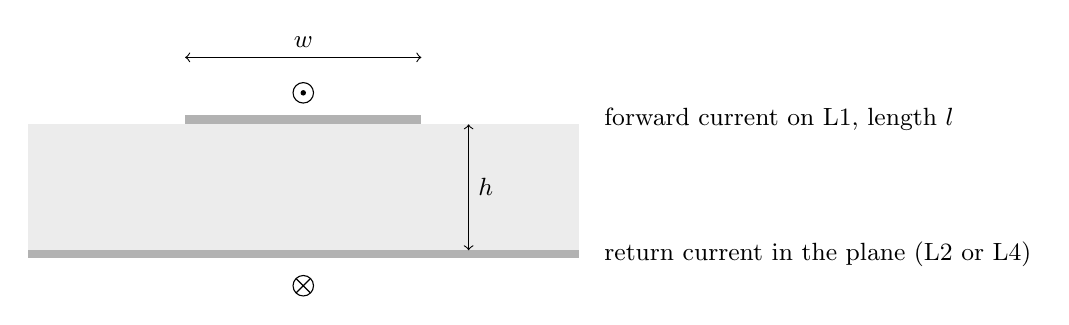
\begin{tikzpicture}[font=\small]
			% laminate, return plane and forward copper (not to scale)
			\fill[gray!15] (0,0) rectangle (7,1.6);
			\fill[gray!60] (0,-0.1) rectangle (7,0);
			\fill[gray!60] (2.0,1.6) rectangle (5.0,1.72);
			% current directions
			\draw (3.5,2.0) circle (0.13); \fill (3.5,2.0) circle (0.035);
			\draw (3.5,-0.45) circle (0.13);
			\draw (3.5,-0.45) ++(-0.09,-0.09) -- ++(0.18,0.18) ++(0,-0.18) -- ++(-0.18,0.18);
			% dimensions
			\draw[<->] (2.0,2.45) -- (5.0,2.45) node[midway, above] {$w$};
			\draw[<->] (5.6,0) -- (5.6,1.6) node[midway, right] {$h$};
			% labels
			\node[anchor=west] at (7.2,1.66) {forward current on L1, length $l$};
			\node[anchor=west] at (7.2,-0.05) {return current in the plane (L2 or L4)};
		\end{tikzpicture}
	\end{center}
	\caption{Cross-section of the power loop: forward copper of width $w$ over a solid return plane at the distance $h$ (not to scale).}
	\label{fig:ex03_loop}
\end{figure}


\subtask{Estimate the loop inductance for both return layers with the parallel-plane formula $L\approx\mu_0hl/w$.}

\begin{solutionblock}
	\begin{equation}
		L_\mathrm{L2} \approx \mu_0\frac{hl}{w} = \SI{1.257}{\nano\henry\per\milli\metre}\cdot\frac{\SI{0.1}{\milli\metre}\cdot\SI{10}{\milli\metre}}{\SI{4}{\milli\metre}} = \SI{0.31}{\nano\henry},\qquad
		L_\mathrm{L4} \approx \SI{4.7}{\nano\henry}.
	\end{equation}
\end{solutionblock}

\subtask{For a strip of width $w$ over a wide plane at the distance $h$ the inductance per length is $L'=Z_0/c_0$, where $Z_0$ is the characteristic impedance of the strip in air ($c_0=\SI{3 \cdot 10^{8}}{\metre\per\second}$). For $w/h\geq1$ (Hammerstad):
\begin{equation*}
	Z_0=\frac{\SI{376.7}{\ohm}}{w/h+1.393+0.667\ln(w/h+1.444)}.
\end{equation*}
Recalculate both cases and explain the difference to the parallel-plane formula.}

\begin{solutionblock}
	L2: $w/h=40$, $Z_0=\SI{8.59}{\ohm}$, $L'=\SI{28.6}{\pico\henry\per\milli\metre}$, $L=\SI{0.29}{\nano\henry}$, i.e.\ 9\,\% below the parallel-plane value.\\
	L4: $w/h=2.67$, $Z_0=\SI{75.3}{\ohm}$, $L'=\SI{0.251}{\nano\henry\per\milli\metre}$, $L=\SI{2.5}{\nano\henry}$, i.e.\ 47\,\% below the parallel-plane value.\\
	The parallel-plane formula assumes that the whole field is confined to the volume $w\cdot h\cdot l$. For $w\gg h$ this holds. For $w/h\approx3$ a large part of the field spreads beside the strip, the effective width is larger than $w$ and the formula overestimates the inductance. The inductance does not depend on the permittivity of the laminate.
\end{solutionblock}

\subtask{With the return on L4 the loop is closed by four vias at each end ($d=\SI{0.3}{\milli\metre}$, length $\SI{1.5}{\milli\metre}$). Estimate the partial inductance of one via and of four vias in parallel. Why is the second value optimistic?}

\begin{solutionblock}
	\begin{equation}
		L_\mathrm{p}\approx\SI{0.2}{\nano\henry\per\milli\metre}\cdot l\left[\ln\frac{4l}{d}-1\right] = \SI{0.2}{\nano\henry\per\milli\metre}\cdot\SI{1.5}{\milli\metre}\cdot(\ln 20-1) = \SI{0.60}{\nano\henry}.
	\end{equation}
	Four vias in parallel give $\SI{0.15}{\nano\henry}$ only if they do not couple. Vias that carry current in the same direction have a positive mutual inductance, so the parallel combination is larger. Interleaving them with vias of the opposite current direction reduces it instead.
\end{solutionblock}

\subtask{The example file \texttt{loop\_L2\_return.inp} (folder \texttt{code/ex03}) describes this loop for the field solver FastHenry, including vias and capacitor pad. It gives $\SI{0.48}{\nano\henry}$ with the return on L2 and $\SI{3.1}{\nano\henry}$ with the return on L4. Which change lowers the inductance of the L4 version most: doubling $w$, halving $l$, or moving the return to L2? Use the strip formula.}

\begin{solutionblock}
	Doubling $w$: $w/h=5.33$, $Z_0=\SI{47.1}{\ohm}$, $L=\SI{1.57}{\nano\henry}$ (factor 1.6 instead of 2, because the field beside the strip does not halve).\\
	Halving $l$: $L=\SI{1.26}{\nano\henry}$ (factor 2).\\
	Return on L2: $L=\SI{0.29}{\nano\henry}$ (factor 8.8).\\
	The distance between forward and return current is the most effective parameter. The field solver confirms the trend; its absolute values are higher because they include the vias, the capacitor pad and the current spreading in the plane.
\end{solutionblock}

%%%%%%%%%%%%%%%%%%%%%%%%%%%%%%%%%%%%%%%%%%%%%%%%%%%%%%%%%%%%%
%% Task 2 %%
%%%%%%%%%%%%%%%%%%%%%%%%%%%%%%%%%%%%%%%%%%%%%%%%%%%%%%%%%%%%%

\task{Loop inductance from a measured ring}

After the turn-on of the high-side switch, the switch-node voltage of a $\SI{48}{\volt}$ GaN half-bridge rings at $f_\mathrm{r0}=\SI{200}{\mega\hertz}$. A $\SI{330}{\pico\farad}$ C0G capacitor is soldered directly across the low-side switch; the ringing frequency drops to $f_\mathrm{r1}=\SI{141}{\mega\hertz}$. The datasheet gives $C_\mathrm{oss}=\SI{300}{\pico\farad}$ at $\SI{48}{\volt}$.

\subtask{Derive the total capacitance $C_\mathrm{par}$ across the low-side switch and the loop inductance from the two measurements. Calculate $Z_0$.}

\begin{solutionblock}
	With $f_\mathrm{r0}=1/(2\pi\sqrt{LC_\mathrm{par}})$ and $f_\mathrm{r1}=1/(2\pi\sqrt{L(C_\mathrm{par}+C_\mathrm{add})})$:
	\begin{equation}
		\left(\frac{f_\mathrm{r0}}{f_\mathrm{r1}}\right)^2 = \frac{C_\mathrm{par}+C_\mathrm{add}}{C_\mathrm{par}}\ \Rightarrow\
		C_\mathrm{par} = \frac{C_\mathrm{add}}{(f_\mathrm{r0}/f_\mathrm{r1})^2-1} = \frac{\SI{330}{\pico\farad}}{2.012-1} = \SI{326}{\pico\farad},
	\end{equation}
	\begin{equation}
		L_\mathrm{loop} = \frac{1}{(2\pi f_\mathrm{r0})^2C_\mathrm{par}} = \SI{1.94}{\nano\henry},\qquad
		Z_0 = \sqrt{\frac{L_\mathrm{loop}}{C_\mathrm{par}}} = \SI{2.44}{\ohm}.
	\end{equation}
\end{solutionblock}

\subtask{$C_\mathrm{par}$ is larger than $C_\mathrm{oss}$. Name possible contributions to the difference. Why must the added capacitor be small and mounted directly across the switch?}

\begin{solutionblock}
	The difference of about $\SI{26}{\pico\farad}$ comes from the switch-node copper over the planes, the winding capacitance of the output inductor, the probe and the tolerance of $C_\mathrm{oss}$.\\
	The added capacitor must carry the ringing current with its own small inductance. An ESL of $\SI{0.4}{\nano\henry}$ makes a $\SI{330}{\pico\farad}$ capacitor appear as $C/(1-\omega^2L_\mathrm{ESL}C)=\SI{368}{\pico\farad}$ at $\SI{141}{\mega\hertz}$. The ring frequency then drops further and the method underestimates $C_\mathrm{par}$ by about 10\,\% (see notebook).
\end{solutionblock}

\subtask{At the turn-on of the high-side switch the switch-node voltage rises linearly within $t_\mathrm{r}$. For an undamped $LC$ circuit the remaining oscillation then has the amplitude $V_\mathrm{DC}\,|\sin x|/x$ with $x=\pi f_\mathrm{r0}t_\mathrm{r}$. Calculate the peak voltage of the low-side switch for $t_\mathrm{r}=1$, 2.5 and $\SI{5}{\nano\second}$.}

\begin{solutionblock}
	\begin{solutiontable}[ht]
		\centering
		\begin{tabular}{lccc}
			\toprule
			$t_\mathrm{r}$                    & $\SI{1}{\nano\second}$ & $\SI{2.5}{\nano\second}$ & $\SI{5}{\nano\second}$ \\
			\midrule
			$x=\pi f_\mathrm{r0}t_\mathrm{r}$ & 0.63                   & 1.57                     & 3.14                   \\
			overshoot $V_\mathrm{DC}|\sin x|/x$ & $\SI{44.9}{\volt}$   & $\SI{30.6}{\volt}$       & $\SI{0}{\volt}$        \\
			peak voltage                      & $\SI{93}{\volt}$       & $\SI{79}{\volt}$         & $\SI{48}{\volt}$       \\
			\bottomrule
		\end{tabular}
		\caption{Turn-on overshoot without damping.}
		\label{stable:ex03_turnon}
	\end{solutiontable}
	An edge that lasts exactly one ringing period ($T_\mathrm{r}=\SI{5}{\nano\second}$) excites no oscillation in this ideal model. In practice the damping and the nonlinear $C_\mathrm{oss}$ reduce the peaks, but a $\SI{100}{\volt}$ device has no margin with the fast edge.
\end{solutionblock}

%%%%%%%%%%%%%%%%%%%%%%%%%%%%%%%%%%%%%%%%%%%%%%%%%%%%%%%%%%%%%
%% Task 3 %%
%%%%%%%%%%%%%%%%%%%%%%%%%%%%%%%%%%%%%%%%%%%%%%%%%%%%%%%%%%%%%

\task{Overshoot at turn-off}

At the turn-off of the high-side switch the load current $I$ has already been taken over by the low-side switch, which clamps the switch node. The channel current of the high-side switch falls linearly from $I$ to zero within $t_\mathrm{f}$ (\autoref{fig:ex03_turnoff}). Use $L_\mathrm{loop}=\SI{1.94}{\nano\henry}$, $C=\SI{326}{\pico\farad}$ and $I=\SI{10}{\ampere}$ from Task 3.2; the circuit is lossless.

%%%%%%%%%%%%%%%%%%%%%%%%%%%%%%%%%%%%%%%%%%%%%%%%%%%%%%%%%%%%%%%%%%%%%%%%%%
% Turn-off model with loop inductance (Exercise 03, Task 3)
%%%%%%%%%%%%%%%%%%%%%%%%%%%%%%%%%%%%%%%%%%%%%%%%%%%%%%%%%%%%%%%%%%%%%%%%%%

\begin{figure}[htb]
	\begin{center}
		\begin{circuitikz}
			\draw (0,0) to[V, l=$V_\mathrm{DC}$] (0,3) to[L, l=$L_\mathrm{loop}$, i>^=$i_L$] (3,3) -- (5,3);
			\draw (3,3) to[I, l_=$i_\mathrm{ch}(t)$] (3,0);
			\draw (5,3) to[C, l=$C$] (5,0);
			\draw (0,0) -- (5,0);
			\draw (3,3) node[circ]{} (3,0) node[circ]{} (5,3) node[circ]{};
			\draw (5,3) node[anchor=south]{A};
		\end{circuitikz}
	\end{center}
	\caption{Turn-off of the high-side switch after the low-side switch has taken over the load current (shown as a short circuit): channel current $i_\mathrm{ch}(t)$, capacitance $C$ across the switch and loop inductance $L_\mathrm{loop}$; $v_\mathrm{DS}=v_\mathrm{A}$.}
	\label{fig:ex03_turnoff}
\end{figure}


\subtask{Show that the overshoot $u=v_\mathrm{DS}-V_\mathrm{DC}$ obeys $\ddot{u}+\omega_0^2u=-\frac{1}{C}\frac{\mathrm{d}i_\mathrm{ch}}{\mathrm{d}t}$ with $\omega_0=1/\sqrt{L_\mathrm{loop}C}$.}

\begin{solutionblock}
	Mesh and node equations: $L_\mathrm{loop}\,\mathrm{d}i_L/\mathrm{d}t=V_\mathrm{DC}-v_\mathrm{DS}=-u$ and $C\,\mathrm{d}u/\mathrm{d}t=i_L-i_\mathrm{ch}$. Differentiating the second equation and inserting the first:
	\begin{equation}
		C\ddot{u} = -\frac{u}{L_\mathrm{loop}} - \frac{\mathrm{d}i_\mathrm{ch}}{\mathrm{d}t}
		\ \Rightarrow\ \ddot{u}+\omega_0^2u = -\frac{1}{C}\frac{\mathrm{d}i_\mathrm{ch}}{\mathrm{d}t}.
	\end{equation}
\end{solutionblock}

\subtask{Solve the equation for the linear current fall with $u(0)=0$ and $\dot{u}(0)=0$. Give $u(t)$ during the fall and the amplitude of the oscillation after it.}

\begin{solutionblock}
	During the fall $\mathrm{d}i_\mathrm{ch}/\mathrm{d}t=-I/t_\mathrm{f}$ is constant:
	\begin{equation}
		u(t) = \frac{I}{\omega_0^2Ct_\mathrm{f}}\left(1-\cos\omega_0t\right) = \frac{L_\mathrm{loop}I}{t_\mathrm{f}}\left(1-\cos\omega_0t\right),\qquad 0\leq t\leq t_\mathrm{f}.
	\end{equation}
	For $t>t_\mathrm{f}$ the circuit oscillates freely. From $u(t_\mathrm{f})$ and $\dot{u}(t_\mathrm{f})$ the amplitude is
	\begin{equation}
		\hat{u} = \frac{L_\mathrm{loop}I}{t_\mathrm{f}}\sqrt{(1-\cos\omega_0t_\mathrm{f})^2+\sin^2\omega_0t_\mathrm{f}} = \frac{2L_\mathrm{loop}I}{t_\mathrm{f}}\left|\sin\frac{\omega_0t_\mathrm{f}}{2}\right|.
	\end{equation}
\end{solutionblock}

\subtask{Show that the amplitude approaches $I\,Z_0$ for $t_\mathrm{f}\rightarrow0$. Evaluate the maximum overshoot for $t_\mathrm{f}=\SI{0.5}{\nano\second}$ and $t_\mathrm{f}=\SI{4}{\nano\second}$ and compare it with $L_\mathrm{loop}I/t_\mathrm{f}$ and $I\,Z_0$.}

\begin{solutionblock}
	For small $t_\mathrm{f}$, $|\sin(\omega_0t_\mathrm{f}/2)|\approx\omega_0t_\mathrm{f}/2$ and $\hat{u}\rightarrow L_\mathrm{loop}I\omega_0=I\sqrt{L_\mathrm{loop}/C}=I\,Z_0=\SI{24.4}{\volt}$. With $\omega_0=\SI{1.257 \cdot 10^{9}}{\per\second}$ ($T_\mathrm{r}=\SI{5}{\nano\second}$):
	\begin{solutiontable}[ht]
		\centering
		\begin{tabular}{lcc}
			\toprule
			$t_\mathrm{f}$                                & $\SI{0.5}{\nano\second}$ & $\SI{4}{\nano\second}$ \\
			\midrule
			$L_\mathrm{loop}I/t_\mathrm{f}$               & $\SI{38.8}{\volt}$       & $\SI{4.9}{\volt}$      \\
			maximum of $u$ during the fall                & $\SI{7.4}{\volt}$        & $\SI{9.7}{\volt}$      \\
			amplitude $\hat{u}$ after the fall            & $\SI{24.0}{\volt}$       & $\SI{5.7}{\volt}$      \\
			\bottomrule
		\end{tabular}
		\caption{Turn-off overshoot without damping, $I\,Z_0=\SI{24.4}{\volt}$.}
		\label{stable:ex03_turnoff}
	\end{solutiontable}
	For the fast fall the overshoot is close to $I\,Z_0$ and $L\,\mathrm{d}i/\mathrm{d}t$ overestimates it by a factor of 1.6. For the slow fall the undamped model gives up to $2L_\mathrm{loop}I/t_\mathrm{f}$; with damping the voltage settles near $L_\mathrm{loop}I/t_\mathrm{f}$. $I\,Z_0$ is an upper bound for any monotonic current fall in the lossless circuit.
\end{solutionblock}

%%%%%%%%%%%%%%%%%%%%%%%%%%%%%%%%%%%%%%%%%%%%%%%%%%%%%%%%%%%%%
%% Task 4 %%
%%%%%%%%%%%%%%%%%%%%%%%%%%%%%%%%%%%%%%%%%%%%%%%%%%%%%%%%%%%%%

\task{RC snubber}

The ring of Task 3.2 shall be damped by an RC snubber across the low-side switch (\autoref{fig:ex03_snubber}). The converter switches at $f_\mathrm{sw}=\SI{1}{\mega\hertz}$.

%%%%%%%%%%%%%%%%%%%%%%%%%%%%%%%%%%%%%%%%%%%%%%%%%%%%%%%%%%%%%%%%%%%%%%%%%%
% Ringing circuit with RC snubber (Exercise 03, Task 4)
%%%%%%%%%%%%%%%%%%%%%%%%%%%%%%%%%%%%%%%%%%%%%%%%%%%%%%%%%%%%%%%%%%%%%%%%%%

\begin{figure}[htb]
	\begin{center}
		\begin{circuitikz}
			\draw (0,0) to[V, l=$V_\mathrm{DC}$] (0,3) to[L, l=$L_\mathrm{loop}$] (3,3) -- (5,3);
			\draw (3,3) to[C, l=$C_\mathrm{par}$] (3,0);
			\draw (5,3) to[R, l=$R_\mathrm{s}$] (5,1.5) to[C, l=$C_\mathrm{s}$] (5,0);
			\draw (0,0) -- (5,0);
			\draw (3,3) node[circ]{} (3,0) node[circ]{};
		\end{circuitikz}
	\end{center}
	\caption{Ringing circuit of the switch that is off ($C_\mathrm{par}=C_\mathrm{oss}+$ layout) with an RC snubber $R_\mathrm{s}$, $C_\mathrm{s}$ across the switch.}
	\label{fig:ex03_snubber}
\end{figure}


\subtask{Choose $C_\mathrm{s}$ as the next E6 value above $3C_\mathrm{par}$ and $R_\mathrm{s}$ as the E12 value closest to $Z_0$.}

\begin{solutionblock}
	$3C_\mathrm{par}=\SI{978}{\pico\farad}$, so $C_\mathrm{s}=\SI{1}{\nano\farad}$; $Z_0=\SI{2.44}{\ohm}$, so $R_\mathrm{s}=\SI{2.2}{\ohm}$.
\end{solutionblock}

\subtask{With $n=C_\mathrm{s}/C_\mathrm{par}$, $r=R_\mathrm{s}/Z_0$ and $p=s/\omega_0$ the characteristic equation of the circuit is $rnp^3+(1+n)p^2+rnp+1=0$. Derive it. For the chosen values the dominant pair of roots gives the damping ratio $\zeta=0.51$ and the natural frequency $\SI{136}{\mega\hertz}$ (see notebook). Interpret the result.}

\begin{solutionblock}
	The node with $C_\mathrm{par}$ and the snubber branch has the admittance $Y=sC_\mathrm{par}+sC_\mathrm{s}/(1+sR_\mathrm{s}C_\mathrm{s})$. The natural frequencies follow from $1+sL_\mathrm{loop}Y=0$:
	\begin{equation}
		s^3L_\mathrm{loop}C_\mathrm{par}R_\mathrm{s}C_\mathrm{s}+s^2L_\mathrm{loop}(C_\mathrm{par}+C_\mathrm{s})+sR_\mathrm{s}C_\mathrm{s}+1=0.
	\end{equation}
	With $s=p\,\omega_0$, $\omega_0^2L_\mathrm{loop}C_\mathrm{par}=1$ and $\omega_0R_\mathrm{s}C_\mathrm{s}=rn$ this becomes $rnp^3+(1+n)p^2+rnp+1=0$.\\
	With $\zeta=0.51$ the amplitude drops to about 2.5\,\% within one period ($e^{-2\pi\zeta/\sqrt{1-\zeta^2}}$) instead of ringing for many periods. The natural frequency drops from $\SI{200}{\mega\hertz}$ to $\SI{136}{\mega\hertz}$ because $C_\mathrm{s}$ partly adds to $C_\mathrm{par}$; the damped oscillation has $\SI{117}{\mega\hertz}$. For $n=3.07$ the maximum damping, $\zeta=0.51$, is reached at $R_\mathrm{s}=0.93\,Z_0$, so the E12 value is close to the optimum.
\end{solutionblock}

\subtask{Estimate the loss of the snubber at $\SI{48}{\volt}$ and compare it with the energy $\frac12L_\mathrm{loop}I^2$ that the ring dissipates per period at $I=\SI{10}{\ampere}$. What do you recommend?}

\begin{solutionblock}
	At each switch-node edge $C_\mathrm{s}$ is charged or discharged through $R_\mathrm{s}$. For edges that are fast compared with $R_\mathrm{s}C_\mathrm{s}=\SI{2.2}{\nano\second}$, this costs $\frac12C_\mathrm{s}V^2=\SI{1.15}{\micro\joule}$ per edge in addition to the losses without snubber (the resistor also absorbs the ring energy, which would otherwise be dissipated elsewhere in the loop):
	\begin{equation}
		\SI{1.15}{\watt}\leq P_\mathrm{s}\leq C_\mathrm{s}V^2f_\mathrm{sw}=\SI{2.3}{\watt},
	\end{equation}
	depending on whether one or both edges are fast. The ring itself dissipates $\frac12L_\mathrm{loop}I^2f_\mathrm{sw}=\SI{0.1}{\watt}$.\\
	Recommendation: reduce $L_\mathrm{loop}$ by layout first (Task 3.1), which lowers $Z_0$ and the overshoot without loss. Use a smaller snubber capacitance only if the overshoot or the EMI spectrum still require it.
\end{solutionblock}

%%%%%%%%%%%%%%%%%%%%%%%%%%%%%%%%%%%%%%%%%%%%%%%%%%%%%%%%%%%%%
%% Task 5 %%
%%%%%%%%%%%%%%%%%%%%%%%%%%%%%%%%%%%%%%%%%%%%%%%%%%%%%%%%%%%%%

\task{Capacitive coupling of the switch node}

A $\SI{400}{\volt}$ half-bridge with 650\,V GaN transistors switches with $\mathrm{d}v/\mathrm{d}t=\SI{100}{\volt\per\nano\second}$ (edge time $\SI{4}{\nano\second}$) at $f_\mathrm{sw}=\SI{500}{\kilo\hertz}$. The high-side transistor is bottom-cooled: its source pad, which is the switch node, is mounted with an area of $\SI{48}{\milli\metre\squared}$ on a $\SI{0.25}{\milli\metre}$ thermal interface ($\varepsilon_\mathrm{r}=6$) on an earthed heat sink.

\subtask{Estimate the capacitance to the heat sink, the common-mode current during an edge and the charge per edge. Where does this current flow?}

\begin{solutionblock}
	\begin{equation}
		C=\varepsilon_0\varepsilon_\mathrm{r}\frac{A}{d}=\SI{8.854}{\pico\farad\per\metre}\cdot6\cdot\frac{\SI{48}{\milli\metre\squared}}{\SI{0.25}{\milli\metre}}=\SI{10.2}{\pico\farad},
	\end{equation}
	$i=C\,\mathrm{d}v/\mathrm{d}t=\SI{1.0}{\ampere}$ during the edge, $Q=CV=\SI{4.1}{\nano\coulomb}$ per edge. The current flows from the heat sink through the protective earth and returns through the mains connection to the converter input: it is common-mode noise, measured by the LISN (L14). In addition, $\frac12CV^2f_\mathrm{sw}=\SI{0.41}{\watt}$ is lost in hard switching.
\end{solutionblock}

\subtask{The low-side transistor is held off through $R_\mathrm{G,off}$ (\autoref{fig:ex03_gate}); $C_\mathrm{GD}=\SI{2}{\pico\farad}$, $C_\mathrm{GS}=\SI{250}{\pico\farad}$, threshold voltage $V_\mathrm{th}=\SI{1.5}{\volt}$ (illustrative). Assume a constant $\mathrm{d}v/\mathrm{d}t=\SI{100}{\volt\per\nano\second}$ and $v_\mathrm{GS}\ll v_\mathrm{DS}$. Derive $v_\mathrm{GS}(t)$ during the edge and evaluate it at the end of the edge for $R_\mathrm{G,off}=\SI{1}{\ohm}$ and $\SI{10}{\ohm}$. Compare with the upper bound for a voltage step.}

%%%%%%%%%%%%%%%%%%%%%%%%%%%%%%%%%%%%%%%%%%%%%%%%%%%%%%%%%%%%%%%%%%%%%%%%%%
% Capacitive coupling of the switch-node edge into the gate (Exercise 03, Task 5)
%%%%%%%%%%%%%%%%%%%%%%%%%%%%%%%%%%%%%%%%%%%%%%%%%%%%%%%%%%%%%%%%%%%%%%%%%%

\begin{figure}[htb]
	\begin{center}
		\begin{circuitikz}
			\draw (3.2,1.6) node[nigfete](Q){};
			\draw (Q.D) -- ++(0,0.6) coordinate (d0) -- ++(0,0.6) node[above]{$v_\mathrm{DS}$, rising with $\mathrm{d}v/\mathrm{d}t$};
			\draw (Q.S) -- ++(0,-0.6) coordinate (s0) -- ++(0,-0.4) coordinate (gnd) node[ground]{};
			\draw (Q.G) -- ++(-1.0,0) coordinate (g0);
			\draw (g0) to[C, l_=$C_\mathrm{GD}$, *-] (g0 |- d0) -- (d0);
			\draw (g0) to[C, l=$C_\mathrm{GS}$] (g0 |- s0) -- (s0);
			\draw (g0) to[R, l=$R_\mathrm{G,off}$] ++(-2.4,0) coordinate (dv) to[sV, l_=0\,V] (dv |- gnd) -- (gnd);
		\end{circuitikz}
	\end{center}
	\caption{Low-side switch, held off by the driver at 0\,V through $R_\mathrm{G,off}$, while the switch node rises.}
	\label{fig:ex03_gate}
\end{figure}


\begin{solutionblock}
	The current $C_\mathrm{GD}\,\mathrm{d}v/\mathrm{d}t$ charges $C_\mathrm{GS}+C_\mathrm{GD}$ and flows out through $R_\mathrm{G,off}$:
	\begin{equation}
		(C_\mathrm{GS}+C_\mathrm{GD})\frac{\mathrm{d}v_\mathrm{GS}}{\mathrm{d}t}+\frac{v_\mathrm{GS}}{R_\mathrm{G,off}}=C_\mathrm{GD}\frac{\mathrm{d}v}{\mathrm{d}t}
		\ \Rightarrow\ v_\mathrm{GS}(t)=R_\mathrm{G,off}C_\mathrm{GD}\frac{\mathrm{d}v}{\mathrm{d}t}\left(1-e^{-t/\tau}\right),\quad\tau=R_\mathrm{G,off}(C_\mathrm{GS}+C_\mathrm{GD}).
	\end{equation}
	$R_\mathrm{G,off}=\SI{1}{\ohm}$: $\tau=\SI{0.25}{\nano\second}$, $v_\mathrm{GS}=\SI{0.2}{\volt}$, safe.\\
	$R_\mathrm{G,off}=\SI{10}{\ohm}$: $\tau=\SI{2.5}{\nano\second}$, $v_\mathrm{GS}(\SI{4}{\nano\second})=\SI{2}{\volt}\cdot(1-e^{-1.59})=\SI{1.59}{\volt}>V_\mathrm{th}$: false turn-on and shoot-through current.\\
	Step bound: $V_\mathrm{DC}C_\mathrm{GD}/(C_\mathrm{GD}+C_\mathrm{GS})=\SI{3.2}{\volt}$. The off path must have a low resistance and, because the edge contains frequencies of several hundred MHz, a low inductance: short gate loop, separate turn-off path, possibly a negative off voltage (L4).
\end{solutionblock}

%%%%%%%%%%%%%%%%%%%%%%%%%%%%%%%%%%%%%%%%%%%%%%%%%%%%%%%%%%%%%
%% Task 6 %%
%%%%%%%%%%%%%%%%%%%%%%%%%%%%%%%%%%%%%%%%%%%%%%%%%%%%%%%%%%%%%

\task{Layout of a half-bridge power loop (homework)}

Lay out the power stage of a $\SI{48}{\volt}$, $\SI{10}{\ampere}$ GaN half-bridge in KiCad on a 4-layer board with the stack-up of Lecture 3 (L1--L2 dielectric $\SI{0.1}{\milli\metre}$). Use two chip-scale GaN transistors, four 0603 input capacitors, the gate driver with its supply capacitor and a footprint for the output inductor.

\subtask{Place the parts and route the power loop and the gate loops. Mark the power loop and its return path in a screenshot of L1 and L2.}

\begin{solutionblock}
	Check list:
	\begin{itemize}
		\item Input capacitors next to the drain of the high-side switch, on L1, each with its own vias to L2.
		\item Return current on L2 directly under the forward path; no slots or splits in L2 under the loop.
		\item Rows of vias between the switches, forward and return vias interleaved.
		\item Driver within a few mm of both gates; gate and Kelvin-source return routed as a pair; driver supply capacitor at the driver pins.
		\item Switch-node area only as large as needed; no ground or signal copper under the high-side driver.
	\end{itemize}
\end{solutionblock}

\subtask{Estimate the loop inductance of your layout with the formulas of Task 3.1. Optionally, adapt \texttt{loop\_L2\_return.inp} to your geometry and compare with FastHenry.}

\begin{solutionblock}
	With the return on L2 and a loop length of about $\SI{10}{\milli\metre}$, values between $\SI{0.3}{\nano\henry}$ and $\SI{0.6}{\nano\henry}$ are realistic, including the packages and the capacitors. A result above $\SI{1}{\nano\henry}$ points to a return path on a distant layer, a long capacitor connection or an interrupted plane.
\end{solutionblock}

\vspace{0.5cm}
Remark: The notebook \texttt{tutorialEx03\_task.ipynb} computes the inductance estimates and simulates the ringing, the turn-off overshoot and the RC snubber of Tasks 3.1 to 3.5.
 % Loop inductance, overshoot, ringing, snubber
	%\include{tex/exercise04} % Gate-loop damping, CSI, bootstrap
	%\include{tex/exercise05} % Probe bandwidth, deskew, efficiency uncertainty
	%\include{tex/exercise06} % Performance factor, optimum flux density, iGSE
	%\include{tex/exercise07} % Dowell, leakage inductance, winding capacitance
	%\include{tex/exercise08} % ZVS timing and energy, TCM, DAB
	%\include{tex/exercise09} % FHA and LLC gain
	%\include{tex/exercise10} % Class E, L-match, wireless power link
	%\include{tex/exercise11} % Charge vectors, SSL and FSL
	%\include{tex/exercise12} % Transfer functions, compensator, loop delay
	%\include{tex/exercise13} % Spectrum envelope, LISN, EMI filter, thermal network
	%\include{tex/exercise14} % Mock oral exam
\end{document}
